\documentclass[aip,amsmath,amssymb,preprint,floatfix]{revtex4-2}

\usepackage{graphicx}
\usepackage{bm}
\usepackage{booktabs}
\usepackage[colorlinks=true,linkcolor=blue,citecolor=blue,urlcolor=blue]{hyperref}

\graphicspath{{../figures/}{figures/}}

\newcommand{\kL}{k_{L}}
\newcommand{\kD}{k_{D}}
\newcommand{\LL}{L_{L}}
\newcommand{\vv}{\bm{v}}
\newcommand{\rr}{\bm{r}}
\newcommand{\zhat}{\hat{\bm{z}}}
\newcommand{\omhat}{\hat{\bm{\omega}}}

\begin{document}

\title{Exact turning invariants for projectile motion under quadratic drag and a
vertical-axis Magnus force}

\author{Pragyaan Gaur}
\email{pragyaangaur12@gmail.com}
\affiliation{Independent researcher}

\date{\today}

\begin{abstract}
A ball spinning about a vertical axis is steered by the Magnus force in the
horizontal plane. We show that for constant lift and drag coefficients this
problem is exactly integrable in its horizontal part: writing the horizontal
velocity as a complex number $w=v_x+iv_y$ and using path length $s$ as the
independent variable, the equation of motion becomes the linear, constant-coefficient
equation $dw/ds=(i\kL-\kD)w$, in which gravity does not appear. Three exact
consequences follow. The heading turns at a constant rate per unit path length,
$d\psi/ds=\kL$, so a $180^\circ$ turn always costs the same path length $\pi \LL$
with $\LL=2m/\rho C_L A$, independently of launch speed, launch angle \emph{and}
drag. The horizontal speed obeys $|w|=|w_0|\exp[-(C_D/C_L)\Delta\psi]$ exactly,
making the horizontal hodograph a logarithmic spiral. The ground-track radius of
curvature is $R_h=\LL\cos\gamma$ with $\gamma$ the flight-path angle, so the track
is an oval whose curvature extremum at apex equals $\LL$. The full system further
collapses to a single scalar ordinary differential equation in the turn angle.
We apply this to a concrete question: can two balls, released simultaneously in
opposite horizontal directions with opposite vertical spin, each turn through
$180^\circ$ and collide head-on at the release height? Without drag the answer is
yes, on a one-parameter family we give in closed form. With drag we show the
launch-to-meeting chord tips below perpendicular by
$(8/3-24/\pi^2)\,\mu\theta^2+O(\mu^2,\theta^4)$, with $\mu=C_D/C_L$; the sign is
positive because $\pi^2>9$, and the rendezvous therefore fails. Numerically the
deficit is strictly positive across $10^{-2}\le\mu\le3$ and $2^\circ\le\theta\le88^\circ$.
Two oppositely thrown balls thus miss by $1$--$46$~m for real sports balls.
All claims are verified against machine-precision numerics; code and data are
openly available.
\end{abstract}

\maketitle

\section{Introduction}
\label{sec:intro}

The lateral deflection of a spinning ball is among the most familiar demonstrations
of fluid dynamics in everyday life, and among the oldest quantitatively studied.
Briggs measured the sideways deflection of a baseball spinning about a
\emph{vertical} axis in a wind tunnel and established its dependence on spin rate
and speed \cite{Briggs1959}; Mehta's review remains the standard entry point to
sports-ball aerodynamics \cite{Mehta1985}; and modern measurements of the lift and
drag coefficients of spinning balls are now routine \cite{Nathan2008,KensrudSmith2018}.

The equations of motion for a spinning ball under gravity, quadratic drag and the
Magnus force are simple to write down and are almost universally integrated
numerically. Bray and Kerwin, in the standard treatment of a soccer ball struck
with sidespin, state the position plainly: ``These equations have no closed form
solutions but can be solved numerically using a Runge--Kutta routine''
\cite{BrayKerwin2003}. Nathan's reference study of baseball flight likewise
proceeds by fourth-order Runge--Kutta \cite{Nathan2008}, as does the recent
pedagogical treatment of Mencke \textit{et al.} \cite{Mencke2020}. In the
projectile-dynamics literature proper, Turkyilmazoglu and Altundag obtain closed
forms when \emph{either} the quadratic drag or the Magnus term is negligible, and
describe the case in which both act simultaneously as highly nonlinear and
admitting only perturbative solutions \cite{Turkyilmazoglu2020}. Chudinov's
asymptotic analysis of the same problem obtains the velocity hodograph only as an
approximate implicit formula \cite{Chudinov2024}. Reviews of projectile motion with
drag \cite{Lubarda2022,Chudinov2022} trace the analytic tradition back to Johann
Bernoulli's 1719 device of parametrising planar motion by the tangent angle rather
than by time, which decouples the equations at the cost of leaving the solution
implicit.

The purpose of this paper is to point out that one physically natural special case
of this system is not merely tractable but exactly integrable in elementary
functions. When the spin axis is vertical and $C_L$, $C_D$ are constant, the
horizontal motion separates completely from gravity and can be solved in closed
form. The resulting invariants are simple, and to our knowledge have not been
recorded.

Section~\ref{sec:model} fixes the model. Section~\ref{sec:reduction} derives the
central identity and the exact reduction of the full nine-dimensional system to a
single scalar equation. Section~\ref{sec:consequences} collects the invariants.
Section~\ref{sec:rendezvous} poses and answers a concrete geometric question that
puts the machinery to work: whether two counter-spinning balls thrown in opposite
directions can be made to collide head-on. Section~\ref{sec:numerics} describes the
numerical verification, and Section~\ref{sec:discussion} discusses scope, an open
problem, and classroom use.

\section{Model}
\label{sec:model}

A ball of mass $m$ and radius $r$, with cross-sectional area $A=\pi r^2$, moves
through still air of density $\rho$ under gravity, quadratic drag, and the Magnus
force,
\begin{equation}
\frac{d\vv}{dt} = -g\zhat
 - \frac{\rho C_D A}{2m}\,|\vv|\,\vv
 + \frac{\rho C_L A}{2m}\,|\vv|\,\bigl(\omhat\times\vv\bigr),
\label{eq:eom}
\end{equation}
where $\omhat$ is the unit spin vector. Throughout we take the spin axis vertical,
$\omhat=\pm\zhat$, which is the pure-sidespin configuration of
Refs.~\onlinecite{Briggs1959} and \onlinecite{BrayKerwin2003}. It is convenient to
absorb the coefficients into two inverse lengths,
\begin{equation}
\kL=\frac{\rho C_L A}{2m},\qquad \kD=\frac{\rho C_D A}{2m},\qquad
\mu\equiv\frac{\kD}{\kL}=\frac{C_D}{C_L},
\label{eq:kdef}
\end{equation}
and to name the \emph{lift length}
\begin{equation}
\LL=\frac{1}{\kL}=\frac{2m}{\rho C_L A}.
\label{eq:LL}
\end{equation}
The combination \eqref{eq:LL} is the exact analogue of the radius of a
constant-$C_L$ turn in aircraft performance, where both the centripetal
requirement and the available lift scale as $v^2$ and the speed cancels.

We write $\psi$ for the azimuth of the horizontal velocity, measured as an unwrapped
angle rather than through an inverse tangent, and $s$ for path length, so that
$ds=|\vv|\,dt$. The flight-path (climb) angle is $\gamma$, with
$\tan\gamma=v_z/|w|$ where $w$ is defined below. Sections~\ref{sec:reduction} and
\ref{sec:consequences} assume $C_L$ and $C_D$ constant; Section~\ref{sec:numerics}
reports what happens when that assumption is relaxed.

\section{Exact reduction}
\label{sec:reduction}

\subsection{The central identity}

Combine the two horizontal components of the velocity into a single complex number,
\begin{equation}
w = v_x + i v_y .
\end{equation}
Three observations make the horizontal problem linear. Gravity is vertical and
contributes nothing to $w$. Drag is antiparallel to $\vv$ and contributes
$-\kD|\vv|w$. And with $\omhat=\zhat$ the Magnus term is
$\omhat\times\vv=(-v_y,\,v_x,\,0)$, which is horizontal and, in complex notation,
is exactly $iw$: a rotation by $90^\circ$. Hence
\begin{equation}
\frac{dw}{dt} = \bigl(i\kL-\kD\bigr)\,|\vv|\,w .
\label{eq:wdot}
\end{equation}
The right-hand side is proportional to $|\vv|$, which is precisely what makes the
change of variable from time to path length effective. Using $ds=|\vv|dt$, the
speed cancels identically and \eqref{eq:wdot} becomes linear with constant
coefficients:
\begin{equation}
\boxed{\;\frac{dw}{ds} = \bigl(i\kL-\kD\bigr)\,w
\quad\Longrightarrow\quad
w(s) = w_0\,e^{-(\kD-i\kL)s}.\;}
\label{eq:master}
\end{equation}
Equation~\eqref{eq:master} is exact. It holds with gravity fully active, at any
launch angle, for any ball, and it is independent of the vertical motion. It is the
source of everything that follows.

Two features are worth emphasising. First, the quadratic velocity dependence of
\emph{both} aerodynamic forces is essential: it is the common factor $|\vv|$ that
cancels under $ds=|\vv|dt$. A Magnus force linear in speed, as arises for vortices
in superfluids where the Magnus--Lorentz correspondence is standard
\cite{Sonin1997}, would not have this property, and the associated turning radius
would depend on speed. Second, the reparametrisation is in the spirit of
Bernoulli's tangent-angle method \cite{Lubarda2022}, but here the angle variable is
an exact affine function of path length, which is what upgrades the solution from
implicit to explicit.

\subsection{Reduction to one scalar equation}

Because $|w(s)|$ is known in closed form, the entire system reduces to a single
scalar equation. Take the turn angle $u\equiv\psi$ as independent variable (by
\eqref{eq:master}, $u=\kL s$) and let
\begin{equation}
Q(u) \equiv \tan\gamma(u) = \frac{v_z}{|w|}.
\end{equation}
Since the Magnus force has no vertical component, $\dot v_z=-g-\kD|\vv|v_z$, and
dividing by $\dot\psi=\kL|\vv|$ gives
$dv_z/du+\mu v_z=-g/(\kL|\vv|)$. Multiplying by the integrating factor $e^{\mu u}$
and using $|w|=|w_0|e^{-\mu u}$ together with $|w|=|\vv|\cos\gamma$ yields
\begin{equation}
\boxed{\;\frac{dQ}{du} = -\lambda\,\frac{e^{2\mu u}}{\sqrt{1+Q^2}},\qquad
Q(0)=\tan\theta,\;}
\label{eq:reduced}
\end{equation}
with the single dimensionless group
\begin{equation}
\lambda = \frac{g}{\kL\,v_0^2\cos^2\theta} = \frac{g\LL}{v_0^2\cos^2\theta},
\label{eq:lambda}
\end{equation}
$\theta$ the launch elevation and $v_0$ the launch speed. Equation~\eqref{eq:reduced}
carries the whole problem: given $Q(u)$, the heading is $\psi=u$, the horizontal
speed is $|w_0|e^{-\mu u}$, the total speed is $|w_0|e^{-\mu u}/\cos\gamma$, and the
position follows by quadrature. A nine-dimensional nonlinear system has been reduced
exactly to one scalar equation in two parameters $(\lambda,\mu)$.

Two functionals of the solution encode the geometry we shall need. Since
$dz/du=v_z/(\kL|\vv|)=\sin\gamma/\kL$, the ball returns to its release height after a
turn $\Psi$ if and only if
\begin{equation}
H \equiv \int_0^{\Psi}\sin\gamma(u)\,du = 0 .
\label{eq:closure}
\end{equation}
Similarly $d(x+iy)/du=w/(\kL|\vv|)=\cos\gamma\,e^{iu}/\kL$, so the launch-to-landing
chord is
\begin{equation}
\text{chord} = \frac{1}{\kL}\int_0^{\Psi}\cos\gamma(u)\,e^{iu}\,du .
\label{eq:chord}
\end{equation}
Equation~\eqref{eq:chord} is exact and is the key formula of
Section~\ref{sec:rendezvous}.

\section{Invariants}
\label{sec:consequences}

\subsection{Constant turning per unit path length}

Taking the argument of \eqref{eq:master},
\begin{equation}
\frac{d\psi}{ds} = \kL = \text{const},
\label{eq:turnrate}
\end{equation}
so the heading advances by a fixed angle per unit distance travelled. Note what is
absent: gravity, launch angle, launch speed, and $C_D$. Drag is antiparallel to
$\vv$ and therefore contributes nothing to $v_xa_y-v_ya_x$; it slows the ball along
the path but cannot bend it. An immediate corollary is that a heading change of
$\Delta\psi$ always costs
\begin{equation}
S = \frac{\Delta\psi}{\kL} = \Delta\psi\,\LL ,
\label{eq:pathlength}
\end{equation}
so in particular a $180^\circ$ turn costs exactly $\pi\LL$ of path, whatever the
launch conditions and whatever the drag. For a baseball with $C_L=0.20$ this is
$\pi\LL=883.6$~m.

\subsection{Logarithmic-spiral hodograph}

Taking the modulus of \eqref{eq:master} and eliminating $s$ using
\eqref{eq:turnrate},
\begin{equation}
|w| = |w_0|\exp\!\bigl[-\mu\,\Delta\psi\bigr],\qquad \mu=\frac{C_D}{C_L},
\label{eq:spiral}
\end{equation}
so the horizontal velocity traces a logarithmic spiral whose pitch is set entirely
by the lift-to-drag ratio. At $\Delta\psi=\pi$ this gives the compact statement
$|w_f|/|w_0|=e^{-\pi C_D/C_L}$. We stress that \eqref{eq:spiral} governs the
\emph{horizontal} speed. The total speed obeys no such law, because gravity
re-accelerates the ball on descent and terminal velocity places a floor under $v_z$;
using $e^{-\pi C_D/C_L}$ for $|\vv_f|/|\vv_0|$ underestimates the true ratio by more
than an order of magnitude at small $C_L/C_D$ (Table~\ref{tab:vf}).

Equation~\eqref{eq:spiral} inverts to
\begin{equation}
\frac{C_D}{C_L} = \frac{\ln\bigl(|w_0|/|w_f|\bigr)}{\Delta\psi},
\label{eq:measure}
\end{equation}
which suggests a measurement: the lift-to-drag ratio of a real ball can be read off
a single tracked trajectory by comparing the decay of its horizontal speed with the
swing of its heading. Gravity drops out of \eqref{eq:measure} identically, so no
correction for the vertical motion is required.

\subsection{Curvature of the ground track}

The radius of curvature of the horizontal projection is
$R_h=(ds_h/dt)/(d\psi/dt)=|w|/(\kL|\vv|)$, and $|w|/|\vv|=\cos\gamma$, so
\begin{equation}
R_h = \LL\cos\gamma .
\label{eq:curvature}
\end{equation}
The track is therefore tightest where the ball is climbing or diving most steeply
and flattest at the apex, where $\gamma=0$ and $R_h=\LL$ exactly. This gives a second
measurement: the radius of curvature of the ground track at the apex is $\LL$
directly, without separate knowledge of $C_L$, $m$ or $A$. In the drag-free case
$\gamma$ runs from $+\theta$ to $-\theta$, so
\begin{equation}
\frac{R_{\max}}{R_{\min}} = \sec\theta ,
\end{equation}
which quantifies exactly how far the track departs from a circle.

\subsection{Gravity is the sole source of non-circularity}

Setting $g=0$ in \eqref{eq:reduced} gives $\gamma\equiv0$, hence $R_h\equiv\LL$: the
ground track is a \emph{perfect circle of radius $\LL$}, whether or not drag is
present. This is a sharper statement than it may appear, since drag can reduce the
speed by any factor without altering the geometry. Table~\ref{tab:circle} confirms
it numerically: a baseball losing $94\%$ of its speed traverses a circle whose fitted
radius agrees with $\LL$ to eleven significant figures.

\begin{table}[t]
\caption{Zero-gravity ground track, fitted circle radius versus $\LL$. Drag changes
the speed by more than an order of magnitude and leaves the radius unchanged.}
\label{tab:circle}
\begin{ruledtabular}
\begin{tabular}{llllll}
ball & drag & fitted radius (m) & $\LL$ (m) & rel.\ error & speed change (m/s) \\
\colrule
baseball & off & 281.267705304 & 281.267705306 & $5.5\times10^{-12}$ & $50\to50.000$ \\
baseball & on  & 281.267705317 & 281.267705306 & $3.8\times10^{-11}$ & $50\to3.200$ \\
frisbee  & off & 8.075877046   & 8.075877046   & $5.4\times10^{-12}$ & $50\to50.000$ \\
frisbee  & on  & 8.075877047   & 8.075877046   & $8.9\times10^{-11}$ & $50\to29.619$ \\
\end{tabular}
\end{ruledtabular}
\end{table}

\begin{figure*}[t]
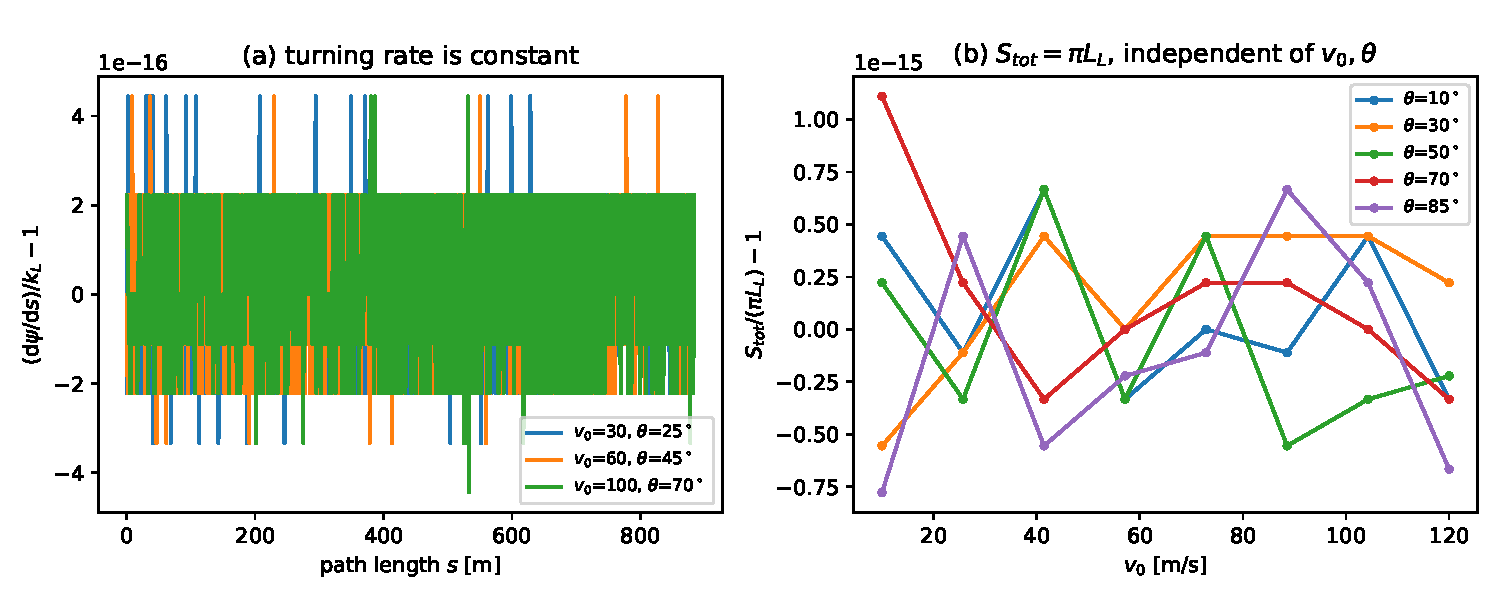
\includegraphics[width=\textwidth]{invariants.pdf}
\caption{Numerical verification of the turning invariants, drag off. Left: the
turning rate $d\psi/ds$ normalised by $\kL$, along the path, for three launch
conditions; the deviation from unity does not exceed $4.4\times10^{-16}$. Right: the
total path length required for a $180^\circ$ turn, normalised by $\pi\LL$, swept over
$v_0\in[10,120]$~m/s at five launch angles; the deviation does not exceed
$1.1\times10^{-15}$.}
\label{fig:invariants}
\end{figure*}

\section{The counter-spinning rendezvous}
\label{sec:rendezvous}

\subsection{Statement}

We now use the machinery on a concrete question. A thrower at the origin releases two
identical balls simultaneously in opposite horizontal directions, one spinning about
$+\zhat$ and the other about $-\zhat$. Both curve in the same sense in the horizontal
plane. Can launch conditions be chosen so that each ball turns through exactly
$180^\circ$ and the two collide head-on at the height of release?

Label the balls $A$ (launched along bearing $0$, spin $+\zhat$) and $B$ (bearing
$\pi$, spin $-\zhat$). The configuration is invariant under reflection in the vertical
plane at bearing $90^\circ$ combined with the exchange $A\leftrightarrow B$, since a
mirror reflection reverses the horizontal velocity and negates the axial spin vector.
Ball $B$'s endpoint is therefore ball $A$'s endpoint reflected in $x$, and the two
coincide if and only if
\begin{equation}
\text{Re}\,(\text{chord}) = 0,
\label{eq:perp}
\end{equation}
that is, if and only if the launch-to-meeting chord is perpendicular to the launch
direction. By \eqref{eq:chord} with $\Psi=\pi$, condition \eqref{eq:perp} reads
\begin{equation}
\mathcal{I} \equiv \int_0^{\pi}\cos\gamma(u)\,\cos u\,du = 0 .
\label{eq:Icond}
\end{equation}
The whole question is the sign of a single integral of a positive weight
$\cos\gamma$ against $\cos u$; the rendezvous succeeds precisely when that weight is
balanced about $u=\pi/2$.

\subsection{Without drag: an exact one-parameter family}

For $\mu=0$ equation \eqref{eq:reduced} is separable, and integrating
$\sqrt{1+Q^2}\,dQ=-\lambda\,du$ gives
\begin{equation}
\tfrac12\bigl[Q\sqrt{1+Q^2}+\operatorname{arcsinh}Q\bigr]
 = \text{const} - \lambda u .
\end{equation}
The map $Q(u)\mapsto -Q(\pi-u)$ preserves the $\mu=0$ equation, so if the solution
satisfies $Q(\pi)=-\tan\theta$ then by uniqueness
\begin{equation}
Q(u) = -\,Q(\pi-u)
\label{eq:antisym}
\end{equation}
identically. Two things follow at once. First, $\sin\gamma$ is odd about $u=\pi/2$,
so the closure condition \eqref{eq:closure} holds automatically. Second,
$\cos\gamma$ is \emph{even} about $u=\pi/2$ while $\cos u$ is odd, so
$\mathcal{I}=0$ exactly: \textbf{without drag the chord is always exactly
perpendicular to the launch direction, at every launch angle.} The rendezvous is
therefore possible, and imposing $Q(\pi)=-\tan\theta$ fixes
\begin{equation}
\lambda = \frac{\tan\theta\sec\theta+\operatorname{arcsinh}(\tan\theta)}{\pi}
        = \frac{f(\theta)}{\pi\cos^2\theta},
\label{eq:lamfree}
\end{equation}
with $f(\theta)=\sin\theta+\cos^2\theta\,\ln(\tan\theta+\sec\theta)$. Combining
\eqref{eq:lamfree} with \eqref{eq:lambda} gives the launch speed in closed form,
\begin{equation}
v_0 = \sqrt{\frac{\pi g \LL}{f(\theta)}} ,
\label{eq:v0}
\end{equation}
for \emph{any} $\theta$: a one-parameter family of solutions. Note that
$f(\theta)v_0^2/g$ is the classical arc length of a drag-free parabola, so
\eqref{eq:v0} simply restates \eqref{eq:pathlength}. For a baseball, \eqref{eq:v0}
ranges from $130.87$~m/s at $\theta=15^\circ$ through a minimum of $85.15$~m/s at
$\theta=60^\circ$; the meeting point lies $515.4$~m away at $\theta=45^\circ$.

A detail worth recording, because it is easy to get wrong: at the meeting point both
balls are \emph{descending}, so their vertical velocities are common-mode and cancel
in the relative velocity. The closing speed is not $2|\vv_f|$ but
\begin{equation}
|\vv_A-\vv_B| = 2|w| = 2\cos\theta\,|\vv_f| ,
\end{equation}
which we confirm numerically to $6.5\times10^{-11}$ relative over
$\theta\in[10^\circ,80^\circ]$. At $\theta=60^\circ$ the closing speed equals a single
ball's speed.

\subsection{With drag: the chord tips below perpendicular}

Once $\mu>0$ the antisymmetry \eqref{eq:antisym} is broken and $\mathcal{I}$ need not
vanish. Because the closure condition \eqref{eq:closure} determines $\lambda$ once
$(\mu,\theta)$ are given, the chord bearing at closure is a function of $(\mu,\theta)$
alone. It cannot depend on $C_L$ and $C_D$ separately, nor on the mass, radius or air
density. This is a theorem, not an observation, and it is confirmed numerically to six
decimal places for coefficient pairs sharing a common $\mu$.

We evaluate the leading behaviour for small drag and small launch angle. Writing
$\beta$ for the chord bearing, a perturbative solution of \eqref{eq:reduced} (see
Appendix~\ref{app:pert}) gives
\begin{equation}
\boxed{\;90^\circ-\beta \;=\; \Bigl(\frac{8}{3}-\frac{24}{\pi^{2}}\Bigr)\mu\,\theta^{2}
 \;+\; O(\mu^{2},\theta^{4})\;}
\label{eq:deficit}
\end{equation}
in radians. The coefficient is
$8/3-24/\pi^2=0.2349583$, and Richardson extrapolation of the numerically computed
deficit reproduces it to a relative accuracy of $7\times10^{-6}$
(Fig.~\ref{fig:deficit}, right panel).

The sign is the point. The coefficient in \eqref{eq:deficit} is positive if and only
if $8/3>24/\pi^2$, that is if and only if
\begin{equation}
\pi^2 > 9 .
\end{equation}
Since $\pi^2=9.8696\ldots$, the deficit is positive, the chord tips below
perpendicular, and the rendezvous fails. It is a pleasant accident that the
obstruction reduces to so elementary an inequality.

\subsection{A tempting argument that does not work}

It is natural to try to prove $\mathcal{I}>0$ pointwise. Folding
\eqref{eq:Icond} about $u=\pi/2$,
\begin{equation}
\mathcal{I} = \int_0^{\pi/2}\bigl[\cos\gamma(u)-\cos\gamma(\pi-u)\bigr]\cos u\,du ,
\label{eq:folded}
\end{equation}
and one might argue that with drag the descent is always steeper than the ascent at
matched turn angle, making the bracket positive everywhere. This is false. Because
drag makes the ascending arc longer than the descending arc, the apex occurs at a
turn angle \emph{greater} than $\pi/2$ (we measure $u_{a}=0.543\pi$, $0.572\pi$ and
$0.635\pi$ for the three cases in Fig.~\ref{fig:deficit}). For $u$ slightly below
$\pi/2$ both $u$ and $\pi-u$ then lie on the ascent, where $|\gamma|$ is decreasing,
so the ordering reverses. The bracket in \eqref{eq:folded} changes sign exactly once
(Fig.~\ref{fig:deficit}, middle panel). The positivity of $\mathcal{I}$ is genuinely
an integral statement, in which a large positive contribution near launch outweighs a
smaller negative one near the midpoint. We record this explicitly because the
pointwise argument is superficially convincing.

\begin{figure*}[t]
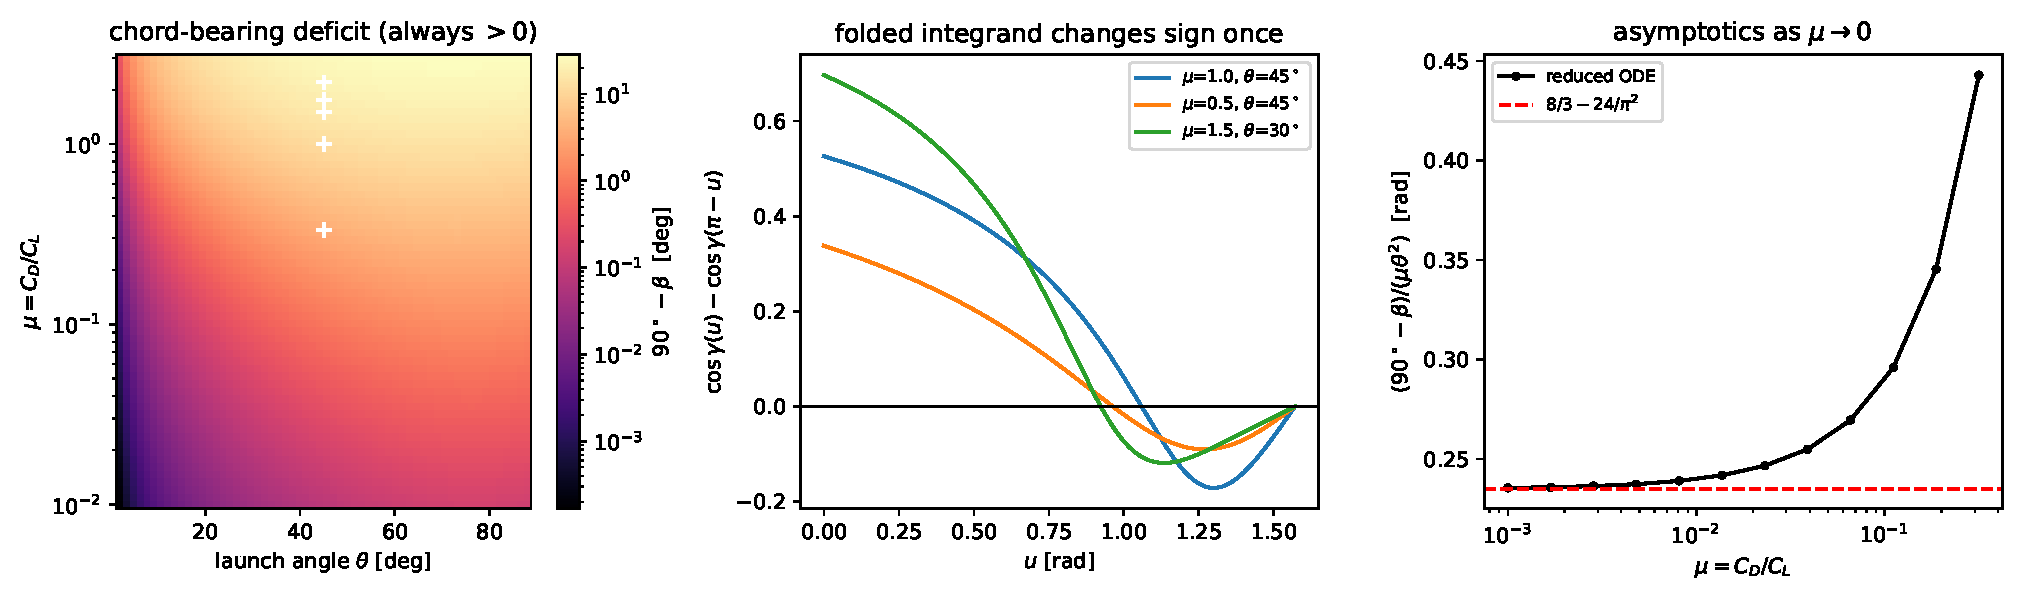
\includegraphics[width=\textwidth]{deficit.pdf}
\caption{The obstruction to the rendezvous, computed from the reduced equation
\eqref{eq:reduced}. Left: the chord-bearing deficit $90^\circ-\beta$ over
$(\mu,\theta)$, strictly positive everywhere, with real sports balls marked at
$\theta=45^\circ$. Middle: the folded integrand of \eqref{eq:folded}, which changes
sign once, showing that the positivity of $\mathcal{I}$ is not pointwise. Right:
convergence of the numerically computed deficit to the analytic coefficient
$8/3-24/\pi^2$ of \eqref{eq:deficit} as $\mu\to0$.}
\label{fig:deficit}
\end{figure*}

\subsection{Numerical survey and consequences}

Beyond the asymptotic regime we evaluate the deficit directly from
\eqref{eq:reduced} over a $60\times60$ grid spanning $10^{-2}\le\mu\le3$ and
$2^\circ\le\theta\le88^\circ$, which brackets every ball in Table~\ref{tab:balls}.
The deficit is strictly positive throughout, with minimum
$1.67\times10^{-4}$ degrees at the corner $\mu=10^{-2}$, $\theta=2^\circ$, where both
small parameters vanish (Fig.~\ref{fig:deficit}, left panel). We therefore state:

\medskip
\noindent\textit{Result.} For constant $C_L$, $C_D$ with $C_D>0$ and a vertical spin
axis, two balls released in exactly opposite horizontal directions with opposite spin
do not collide, at any launch speed or launch angle. This is proved for small
$\mu\theta^2$ by \eqref{eq:deficit} and established numerically over the physically
relevant domain; a proof for all $(\mu,\theta)$ remains open.
\medskip

The practical size of the failure is not small. The two balls miss by
$2|\text{chord}|\cos\beta$, which for the closure solutions of
Table~\ref{tab:balls} is $1.0$--$1.9$~m for a frisbee, $7.6$--$9.4$~m for a table
tennis ball and $30$--$46$~m for a soccer ball.

We note in passing that this changes the count of conditions. The two residuals
``return to launch height'' and ``$\psi=\pi$'' are two ways of writing the single
scalar statement that two events coincide, over the three unknowns $(v_0,\theta,t^*)$;
the corresponding $2\times2$ Jacobian is numerically rank one, with singular-value
ratio $4.0\times10^{-9}$. The physical problem nevertheless becomes genuinely
two-dimensional once drag is present, through the independent condition
\eqref{eq:perp}, which without drag is satisfied automatically.

\section{Numerics and validation}
\label{sec:numerics}

The full system is integrated as an eleven-component state
$[\rr,\vv,\bm{\omega},\psi,s]$, carrying $\psi$ and $s$ as state variables so that the
heading unwraps correctly past $\pm\pi$ without any inverse-tangent differencing.
Integration uses explicit Runge--Kutta 4(5) with relative tolerance $10^{-10}$ and
event detection for the two closure events, never fixed steps
\cite{Virtanen2020,Harris2020}. Parameter sweeps use a batched fixed-step
integrator. Figures are produced with Matplotlib \cite{Hunter2007}.

Table~\ref{tab:verify} summarises the verification. The reduced equation
\eqref{eq:reduced} reproduces $\gamma(\psi)$ from the full three-dimensional
integration to better than $10^{-8}$~rad across four balls and three launch angles,
and the reduced chord bearing agrees with the full simulation to better than
$10^{-4}$ degrees. The invariants \eqref{eq:turnrate} and \eqref{eq:pathlength} hold
to machine precision. Crucially, \eqref{eq:turnrate} holds equally with drag active,
confirming that drag cannot torque the azimuth.

\begin{table}[t]
\caption{Verification of the analytic results against direct integration. Deviations
are relative unless stated.}
\label{tab:verify}
\begin{ruledtabular}
\begin{tabular}{lll}
quantity & condition & max deviation \\
\colrule
$d\psi/ds=\kL$                        & drag off & $4.4\times10^{-16}$ \\
$d\psi/ds=\kL$                        & drag on  & $6.7\times10^{-16}$ \\
$S_{\rm tot}=\pi\LL$                  & drag off, $v_0\times\theta$ sweep & $1.1\times10^{-15}$ \\
$|w|=|w_0|e^{-\mu\Delta\psi}$         & drag on, four balls & $<10^{-9}$ \\
$R_h=\LL\cos\gamma$                   & drag on and off & $<10^{-12}$ \\
$g=0$ track is a circle of radius $\LL$ & drag on and off & $<10^{-9}$ \\
reduced ODE vs.\ full 3-D $\gamma(\psi)$ & drag on, four balls & $<10^{-8}$~rad \\
$\lambda$ from \eqref{eq:lamfree}     & drag off & $3.5\times10^{-12}$ \\
$v_0$ from \eqref{eq:v0}              & drag off & $2\times10^{-14}$ \\
closing speed $=2\cos\theta|\vv_f|$   & drag off & $6.5\times10^{-11}$ \\
$R_{\max}/R_{\min}=\sec\theta$        & drag off & $<10^{-6}$ \\
\end{tabular}
\end{ruledtabular}
\end{table}

\subsection{Beyond constant coefficients}

The results of Sections~\ref{sec:reduction} and \ref{sec:consequences} require
$C_L$ and $C_D$ constant. Two remarks bound their scope. First, under constant $C_L$
the Magnus term depends on the spin \emph{direction} only, so the spin magnitude is
exactly inert: trajectories for $\omega=50$, $200$ and $800$~rad/s coincide to twelve
digits. Any question about sensitivity to spin rate is therefore empty until $C_L$ is
allowed to depend on the spin parameter $S=r\omega/|\vv|$. With the saturating form
$C_L=1/(2+1/S)$, a $10\%$ spin mismatch between the two balls produces a $1084$~m
miss at the drag-free $45^\circ$ solution, larger than the chord itself. Second, we
have implemented a smoothed drag-crisis model in which $C_D$ falls from $0.47$ to
$0.15$ across $\mathrm{Re}\sim2$--$4\times10^5$; with $C_D$ varying, $|w|$ no longer
follows \eqref{eq:spiral} exactly, though \eqref{eq:turnrate} survives so long as
$C_L$ is constant, since drag never contributes to the turning rate whatever its
magnitude.

\subsection{Real balls}

Table~\ref{tab:balls} collects the closure solutions with drag active, using
representative coefficients \cite{Mehta1985,Nathan2008,KensrudSmith2018}. Only three
of six objects can complete a $180^\circ$ turn at all below $150$~m/s: the required
path $\pi\LL$ must be covered before drag exhausts the ball. A baseball manages
$0.504\pi$ of turn at best, falling short by $0.496\pi$; a solution exists
mathematically only near $v_0=616$~m/s, which is Mach~$1.8$ and outside the validity
of an incompressible quadratic-drag model. We emphasise, in view of
Section~\ref{sec:rendezvous}, that the entries in Table~\ref{tab:balls} are
single-ball $180^\circ$ closures and are \emph{not} rendezvous solutions.

\begin{table}[t]
\caption{Closure of a single $180^\circ$ turn with drag active, $v_0$ capped at
$150$~m/s; the minimum-$v_0$ member of the $\theta$-family is shown. Coefficients are
representative constants, not measurements.}
\label{tab:balls}
\begin{ruledtabular}
\begin{tabular}{lcccccc}
object & $C_L/C_D$ & closes & $\theta$ & $v_0$ (m/s) & $t$ (s) & $v_f/v_0$ \\
\colrule
frisbee   & 3.00  & yes & $64^\circ$ & 19.85  & 2.813 & 0.590 \\
soccer    & 1.00  & yes & $76^\circ$ & 124.20 & 9.583 & 0.211 \\
table tennis & 0.667 & yes & $80^\circ$ & 90.95  & 3.966 & 0.096 \\
golf      & 1.00  & no  & --- & --- & --- & $\psi_{\max}=0.804\pi$ \\
baseball  & 0.571 & no  & --- & --- & --- & $\psi_{\max}=0.504\pi$ \\
tennis    & 0.455 & no  & --- & --- & --- & $\psi_{\max}=0.565\pi$ \\
\end{tabular}
\end{ruledtabular}
\end{table}

\begin{table}[t]
\caption{Residual speed at closure: the exact horizontal law \eqref{eq:spiral}
compared with the same expression applied, incorrectly, to the total speed.}
\label{tab:vf}
\begin{ruledtabular}
\begin{tabular}{lll}
$C_L/C_D$ & $e^{-\pi C_D/C_L}$ & simulated $|\vv_f|/|\vv_0|$ \\
\colrule
0.5  & 0.0019 & 0.0435 \\
1.0  & 0.0432 & 0.2110 \\
2.0  & 0.2079 & 0.4622 \\
3.0  & 0.3509 & 0.5938 \\
5.0  & 0.5335 & 0.7263 \\
10.0 & 0.7304 & 0.8506 \\
\end{tabular}
\end{ruledtabular}
\end{table}

\begin{figure}[t]
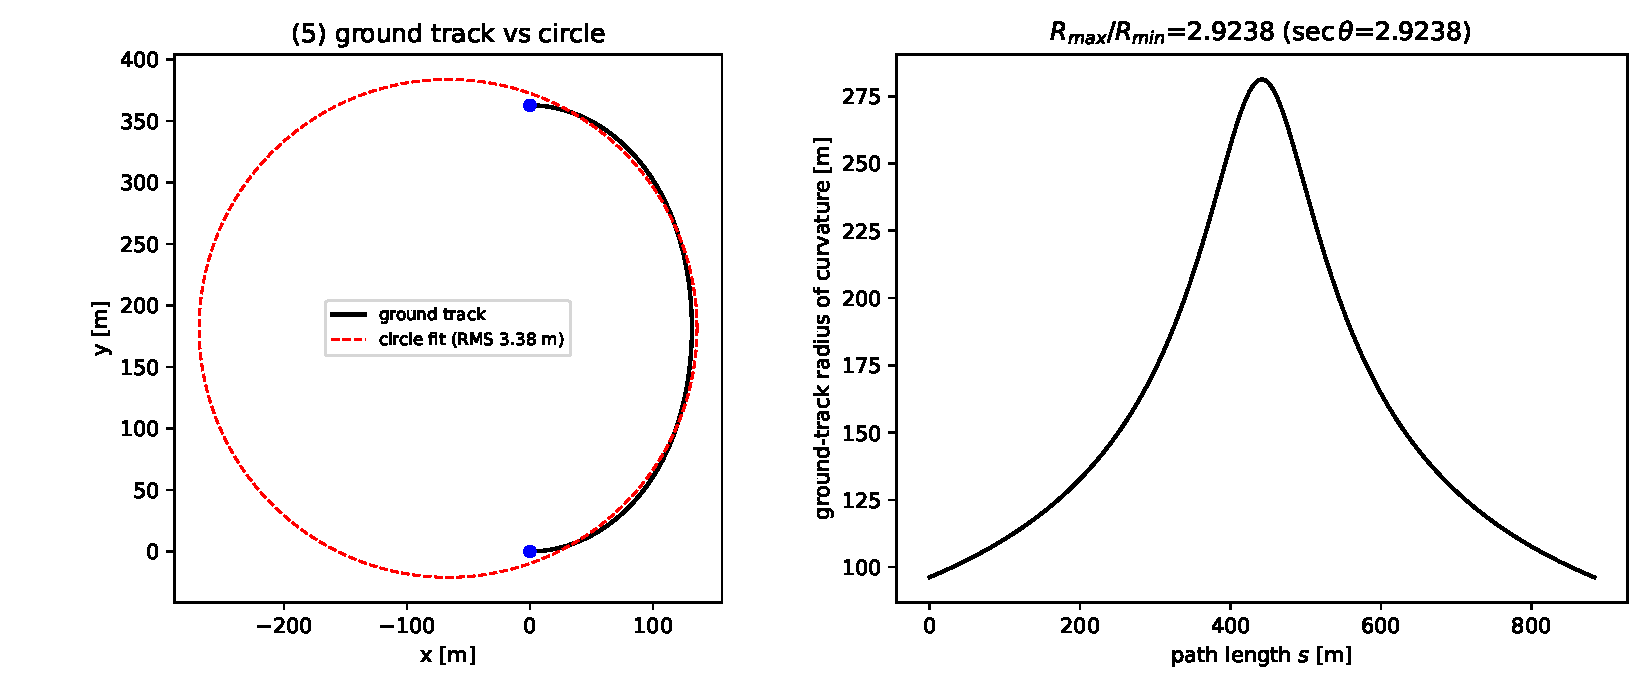
\includegraphics[width=\columnwidth]{ground_track.pdf}
\caption{Ground track of a drag-free closure solution at $\theta=45^\circ$. Left: the
track against its best-fit circle; the RMS residual is $1.585$~m on a fitted radius of
$264.06$~m, which is $43$ times the ball radius. Right: the radius of curvature along
the path, following $R_h=\LL\cos\gamma$ with $R_{\max}/R_{\min}=\sec\theta$.}
\label{fig:shape}
\end{figure}

\begin{figure}[t]
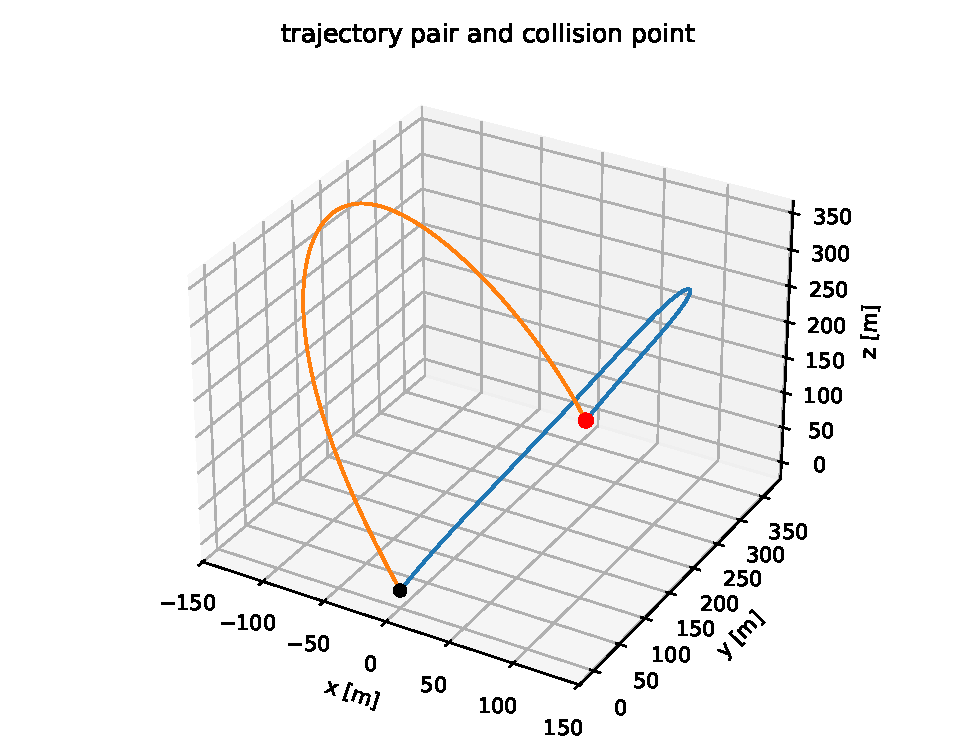
\includegraphics[width=\columnwidth]{trajectory_pair.pdf}
\caption{The drag-free rendezvous: the two counter-spinning trajectories and their
common endpoint, at $\theta=45^\circ$ for a baseball. The mirror symmetry is exact,
with arrival times agreeing to $3.6\times10^{-15}$~s.}
\label{fig:pair}
\end{figure}

\section{Discussion}
\label{sec:discussion}

\subsection{Relation to known results}

The individual ingredients here are old. The complex substitution $w=v_x+iv_y$ is
standard for rotating-frame problems; the constant-$C_L$ turn radius $2m/\rho C_L A$
is the aircraft-performance result that a wing at fixed lift coefficient turns with a
speed-independent radius; and the reparametrisation of projectile motion by a
geometric angle is Bernoulli's, dating to 1719 \cite{Lubarda2022}. What appears not to
have been noticed is that these combine, for the vertical-axis case specifically, into
an exactly solvable system: the turning angle is an affine function of path length, so
Bernoulli's implicit solution becomes explicit, and the turn radius survives the
addition of drag untouched.

It is worth being precise about why the vertical-axis case is special and the general
one is not. For a general spin orientation the Magnus term is not a pure rotation of
$w$, the horizontal equation does not close, and \eqref{eq:master} fails; this is
consistent with the perturbative status of the general problem in
Ref.~\onlinecite{Turkyilmazoglu2020}. In exterior ballistics the situation is
different again: for spin-stabilised projectiles the Magnus \emph{force} is usually
small enough to neglect and the relevant lateral deflection arises from the Magnus
moment through the yaw of repose \cite{McCoy2012}, a gyroscopic mechanism unrelated
to the one considered here.

The Magnus--Lorentz analogy familiar from vortex dynamics \cite{Sonin1997} is
instructive precisely where it breaks. There the Magnus force is linear in velocity,
exactly like the Lorentz force, and the resulting circular orbits have radius
proportional to speed. The aerodynamic Magnus force is quadratic, and the radius is
$\LL$ regardless of speed. The speed-independence is what makes \eqref{eq:pathlength}
possible.

\subsection{An open problem}

If one drops the requirement that each ball turn through exactly $180^\circ$ and asks
only that two oppositely thrown balls collide head-on at release height, the
head-on condition becomes
\begin{equation}
\Delta\psi_A+\Delta\psi_B = 2\pi ,
\end{equation}
so that the \emph{sum} of the turns is fixed while the split need not be equal; the
equal split is a drag-free accident. Counting gives four unknowns
$(v_{0A},\theta_A,v_{0B},\theta_B)$ against four conditions, suggesting isolated
solutions with one ball turning past $180^\circ$. We searched for these over a
$70\times70$ grid with pairing restricted to $\Delta\psi_A<\pi<\Delta\psi_B$ and found
candidates with genuinely unequal turns ($145^\circ$ and $215^\circ$), but every
refinement drained back to the degenerate corner $\theta\to0$, $v_0\to\infty$ and
stalled at a residual miss of $1.5$--$2.0$~mm consistent with the $\theta^2$ law of
\eqref{eq:deficit}. We were unable to establish either existence or non-existence of a
finite-angle asymmetric solution, and record it as open.

\subsection{Classroom use}

Several of these results are accessible as exercises. Deriving \eqref{eq:master} from
\eqref{eq:eom} requires only the observation that $\omhat\times\vv$ is a rotation, and
makes an unusually clean illustration of why choosing the right independent variable
matters. The statement that a $180^\circ$ turn costs a fixed distance regardless of
how hard the ball is thrown is counter-intuitive enough to be worth setting before the
derivation. The $g=0$ circle of Table~\ref{tab:circle} is a good computational
exercise, as is verifying that drag does not appear in \eqref{eq:turnrate}. Finally,
Section~\ref{sec:rendezvous}~D is a useful cautionary example of a plausible pointwise
argument that fails, with the failure diagnosable by plotting one function.

\begin{acknowledgments}
The author thanks the maintainers of SciPy, NumPy and Matplotlib.
\end{acknowledgments}

\section*{Data availability}

The complete source code, regression test suite and figure-generating scripts are
openly available \cite{ThisCode}. All numbers quoted in this paper are reproduced by
a single driver script, and the analytic claims are encoded as regression tests with
the tolerances stated in Table~\ref{tab:verify}.

\appendix

\section{Leading-order deficit}
\label{app:pert}

We sketch the calculation leading to \eqref{eq:deficit}. Work to first order in $\mu$
and second order in $\theta$. For small $Q$, \eqref{eq:reduced} linearises to
$Q'\simeq-\lambda(1+2\mu u)$, so
\begin{equation}
Q(u) \simeq \theta - \lambda\bigl(u+\mu u^2\bigr).
\end{equation}
Imposing closure \eqref{eq:closure}, $\int_0^\pi Q\,du=0$ at this order, gives
\begin{equation}
\lambda = \frac{\theta}{\pi/2+\mu\pi^2/3}
        \simeq \lambda_0\Bigl(1-\frac{2\pi\mu}{3}\Bigr),\qquad
\lambda_0=\frac{2\theta}{\pi}.
\end{equation}
With $\cos\gamma\simeq1-Q^2/2$ and $\int_0^\pi\cos u\,du=0$,
\begin{equation}
\mathcal{I} \simeq -\tfrac12\int_0^\pi Q^2\cos u\,du .
\end{equation}
Using $\int_0^\pi u\cos u\,du=-2$, $\int_0^\pi u^2\cos u\,du=-2\pi$ and
$\int_0^\pi u^3\cos u\,du=12-3\pi^2$, and expanding to first order in $\mu$, the
terms independent of $\mu$ cancel identically (as they must, by \eqref{eq:antisym}),
leaving
\begin{equation}
\int_0^\pi Q^2\cos u\,du \simeq
 \mu\theta^2\Bigl(\frac{16}{3}-16+\frac{96}{\pi^2}\Bigr).
\end{equation}
The imaginary part of \eqref{eq:chord} is $\int_0^\pi\cos\gamma\sin u\,du\simeq2$ at
leading order, so
\begin{equation}
90^\circ-\beta \simeq \frac{\mathcal{I}}{2}
 = \mu\theta^2\Bigl(\frac{8}{3}-\frac{24}{\pi^2}\Bigr),
\end{equation}
which is \eqref{eq:deficit}. The coefficient is positive because $\pi^2>9$.

\bibliography{refs}

\end{document}
